\chapter{Background Knowledge}\label{chapter:background-knowledge}

In this chapter, we will explore some of the background knowledge required to understand the methodology chosen and experiments undertaken throughout this thesis.
We will first explore Variable Autoencoders before delving into some background about Reinforcement Learning and a discussion of Wi-Fi Channel State Information (CSI) and Body-coordinate Velocity Profiles (BVP).
Finally, we will discuss the three signal-to-image transformations that are explored in this work.

\section{Variational Autoencoders}

Variational autoencoders (VAEs) are a type of generative model which combines elements of both autoencoders and probabilistic modeling and are suited for unsupervised learning and representation learning and was first introduced by Kingma and Weling in \cite{kingma2013auto}.
Standard autoencoders are a network architecture in which data is encoded into a lower-dimensional latent space by an encoder.
A decoder then reconstructs the original input from the latent representation.
VAEs introduce probabilistic modeling to autoencoders by using a probability distribution over the latent space instead of using the latent space directly.

Its original design aimed at using a generative model as an implicit form of regularization.
By forcing the model to learn a representation which is also useful for data generation, the representation learned must have some sort of statistically independent but meaningful representation of the variations in the input data, leading to better performance at both the auxiliary task of data generation as well as the main task of discrimination \cite{kingma2019introduction}.

Generally, VAEs are described as two coupled but independent models: the encoder and decoder.
The encoder is a Bayesian network of the form $q(\boldsymbol{z} | \boldsymbol{x})$ where $\boldsymbol{z}|\boldsymbol{x}$ may be a (deep) neural network.
Similarly, the decoder is also a Bayesian network of the form $p(\boldsymbol{x}|\boldsymbol{z}) p(\boldsymbol{z})$ where $\boldsymbol{x}|\boldsymbol{z}$ may also be a (deep) neural network.
The input signal $\boldsymbol{x}$ is thus represented by $\boldsymbol{z}$.

The purpose of the encoder $q_\phi(\boldsymbol{z}|\boldsymbol{x})$ with parameters $\phi$ is to produce an approximation of the true, but intractable, posterior.
The encoder neural network is then used to produce the set of parameters for latent variables such that

\begin{align}
	(\boldsymbol{\mu}, \log \boldsymbol{\sigma}) &= \text{EncoderNeuralNet}_\phi (\boldsymbol{x})\\
	q_\phi(\boldsymbol{z}|\boldsymbol{x}) &= \mathcal{N}(\boldsymbol{z}; \boldsymbol{\mu}, \text{diag}(\boldsymbol{\sigma}))
\end{align}
where $\mathcal{N}$ is the normal distribution.

The purpose of the decoder $p_\theta (\boldsymbol{x}|\boldsymbol{z})$ is to produce a mapping between the latent space $p_\theta (\boldsymbol{z})$ and the original, observed distribution through learning a joint distribution $p_\theta (\boldsymbol{x}, \boldsymbol{z}) = p_\theta (\boldsymbol{z})p_\theta (\boldsymbol{x}|\boldsymbol{z})$.

The VAE is optimized through the evidence lower bound (ELBO), incorporating Kullback-Leibler divergence, the details of which are thoroughly explained in \cite{kingma2019introduction}.

By using the reparameterization trick introduced in \cite{kingma2013auto}, the ELBO can then be differentiated with respect to both parameters $\phi$ and $\theta$ at the same time through stochastic gradient descent.

VAEs are used in various areas including image generation, data compression, denoising, and image recognition.
By using a latent representation of the data which is statistically meaningful, the generated data is much more likely to come from the same underlying distribution as the original data.

\section{Reinforcement Learning} \label{sec:background-rl}

Reinforcement learning (RL) is a machine learning paradigm which teaches agents how to make decision in complex environments \cite{tavakol2022dic}.
The general paradigm is that of an agent which takes actions in an environment as a response to its observations of the current environment state.
The environment then provides a reward for the agent and transitions into a new state as a response to the action.
The agent is given the goal of maximizing the cumulative reward over time.
The main use cases of RL are in robotics, gaming, finance, and healthcare where performing complex tasks or optimizing control systems is necessary.

Throughout this work, we focus on model-free RL.
Model-free RL is an approach to RL which focuses on learning directly from interactions with the environment without necessarily modeling the dynamics of the environment explicitly.
With this approach, the agent learns policies or value functions which it uses to make decisions.
Some well-known model-free RL algorithms include Q-Learning, State-Action-Reward-State-Action (SARSA), Deep Q-Networks (DQN), Proximal Policy Optimization (PPO), and Asynchronous Advantage Actor-Critic (A3C).

Furthermore, there are two main learning paradigms to RL, namely on- and off-policy learning.

On-policy RL learns directly from data collected by the current policy.
This entails updating the policy directly using data, i.e., the reward gathered, of the same policy.
This makes it especially suitable for scenarios where data collection is cheap, for whatever measure of cheap is appropriate in the given scenario.
By updating the policy directly, the learning trajectory may be more stable due to consistency.
On the other hand, this same consistency can lead to reduced exploration of the action space as well as reduced sample efficiency due to the slow exploration.
An example of this learning paradigm is PPO, which is one of the two methods used in this thesis.

Off-policy RL, conversely, learns from a \textit{replay buffer} of past experiences.
A replay buffer is a store of past experiences that an agent has experienced.
During each step taken where the agent interacts with its environment, the action and resulting observation and reward is stored.
During the update stage, a random sampling from the replay buffer is then taken and used to update the agent's policy or value function.
By doing so, this enables \textit{off-policy} learning, where the agent learns from previous experiences, including those performed under a different policy.
This also allows for updates to be performed in batches, increasing throughput.
The increased data diversity and ability to use samples from previous policies leads to better exploration and better sample efficiency.
One example of off-policy RL is Deep Deterministic Policy Gradient (DDPG).

\subsection{Proximal Policy Optimization}\label{subsec:background-ppo}

PPO is a model-free on-policy RL algorithm proposed in Schulman et al. \cite{schulman2017proximal}.
It is a further development based on Trust Region Policy Optimization (TRPO) \cite{schulman2017trust} and works by iteratively sampling data through interactions with the environment and optimizing a ``surrogate'' objective function using stochastic gradient ascent. The paper explores two approaches to this ``surrogate'' function, one using a penalty on KL divergence and one using a clipped objective function.

In the KL divergence approach, for each update of a given policy $\pi_\theta$, the KL-penalized objective $L^{KLPEN}$ is optimized with

\begin{equation}
	L^{KLPEN}(\theta) = \hat{\mathbb{E}}_t \left[\frac{\pi_\theta(a_t | s_t)}{\pi_{\theta_{old}} (a_t | s_t)} \hat{A}_t - \beta KL \left( \pi_{\theta_{old}} (\cdot | s_t), \pi_\theta(\cdot | s_t)\right) \right]
\end{equation}
where $t$ is the current timestep, $a$ the action, $s$ the environment state, $\hat{A}_t$ an estimator of the advantage function at timestep $t$, and $\hat{\mathbb{E}}_t$ the empirical average over a finite batch of samples.
With every policy update, we also update $\beta$ by first computing $d = \hat{\mathbb{E}}_t\left(\pi_{\theta_{old}} (\cdot | s_t), \pi_{\theta}(\cdot | s_t)\right)$.
If $d < d_{targ} / 1.5$, then we half $\beta$.
If $d > d_{targ} \times 1.5$, then we double $\beta$. $\beta$ is a hyperparemter that can be chosen, but is ``not important in practice because the algorithm quickly adjusts it'' \cite{schulman2017proximal}.

In the clipped surrogate objective approach, for each update of the policy, the clipped surrogate objective $L^{CLIP}$ for a given policy $\pi_\theta$ is updated, where

\begin{align}
	L^{CLIP}(\theta) &= \min \left[ 
		\frac{\pi_\theta(a_t | s_t)}{\pi_{\theta_{old}} (a_t | s_t)} \hat{A}_t, g(\epsilon, \hat{A}_t)
	\right]\\
	\text{where } g(\epsilon, \hat{A}_t) &= \begin{cases}
		(1 + \epsilon) \cdot \hat{A}_t & \hat{A}_t \geq 0 \\
		(1 - \epsilon) \cdot \hat{A}_t & \hat{A}_t < 0
	\end{cases}
\end{align}

The clipped surrogate object approach shows better empirical performance in \cite{schulman2017proximal} and is the one that we use in this thesis.

The algorithm itself is relatively simple and is best understood by directly reading the pseudocode seen in Algorithm \ref{algo:ppo}.

\begin{algorithm}
	\SetAlgoLined
	\KwIn{Initialize policy parameters $\theta_0$ and value function parameters $\phi_0$}
	\For{$k=0, 1, 2,\ldots$}{
		Collect trajectories ${D}_k = \{\tau_i\}$ by running policy $\pi_k=\pi_{\theta_k}$ in the environment\;
		Compute rewards $\hat{R}_t$ for each action\;
		Calculate advantage estimates $\hat{A}_t$ using the value function $V_{\phi_k}$\;
		Update the policy by maximizing $L^{CLIP}$:
		\begin{equation}
			\theta_{k+1} = \arg \underset{\theta}{\min} \frac{1}{|{D}_k|T} \sum_{\tau \in {D}_k} \sum_{t=0}^{T} L^{CLIP} 
		\end{equation}
		using Adam\;
		Fit the value function by regression on mean-squared error over the collected trajectories ${D}_k$\;
	}
	\caption{Proximal Policy Optimization (PPO) Algorithm}\label{algo:ppo}
\end{algorithm}

\subsection{Deep Q-Networks}

Before we delve into DDPG, we will firsts look at DQNs, which DDPG builds off of and extends to continuous action spaces.
DQNs is a model-free off-policy RL alrogithm and is an extension of Q-Learning which replaces the crafted Q-tables with neural networks \cite{watkins1989learning,mnih2015human}.

The concept behind DQNs is to use a deep neural network to approximate the optimal action-value function
\begin{equation}
	Q^* (s, a) = \underset{\pi}{\max} \mathbb{E}\left[r_t + \gamma r_{t+1} + \gamma^2 r_{t+2} + \ldots | s_t=s, a_t=a, \pi\right]
\end{equation}
where $r_t$ is the reward at time $t$, $\gamma$ a hyperparameter, $\pi=P(a|s)$ the policy, and $s, a$ the observation and action, respectively.
Intuitively, $Q^*$ then is the maximum sum of rewards discounted by $\gamma$ after making a given observation and taking a given action.

The agent's experiences $e_t = (s_t, a_t, r_t, s_{t+1})$ are stored in the replay buffer $D_t\{e_1,\ldots,e_t\}$.
The Q-network is then updated during the learning process in batches of randomly and uniformly sampled experiences from $D$ such that the drawn samples are $(s,a,r,s') \sim U(D)$.
A separate target network is introduced as well to address the problem of instability during training.
The target network is a copy of the Q-network, but is updated less frequently and often with a slower learning rate.

At each iteration $i$ of the learning process, the loss function which is optimized for is the Bellman equation describing the optimal action-value function and is given by
\begin{equation}
	L_i(\theta_i) = \mathbb{E}_{(s,a,r,s') \sim U(D)} \left[\left(
		r + \gamma \underset{a'}{\max}Q(s', a'; \theta_i^-) - Q(s,a; \theta_i)
	\right)^2\right]
\end{equation}
where $\theta_i$ are the parameters of the Q-network at iteration $i$ and $\theta_i^-$ are the target network parameters.
$\theta_i^-$ are only updated with the Q-network parameters $\theta_i$ every $C$ steps and are otherwise kept fixed.


\subsection{Deep Deterministic Policy Gradient}\label{subsec:background-ddpg}

DDPG builds on DQNs and extends the action space to continuous action spaces \cite{lillicrap2015continuous}.
Extending the action space by simply discretizing a continuous action space is not viable due to the curse of dimensionality that comes with too many output dimensions.
DDPG provides a solution by concurrently learning a Q-function, called the critic, as well as a policy, called the actor.

The loss function optimized by the critic in DDPG is modified from DQN to include the actor such that
\begin{align}
	L_Q &= \frac{1}{N}\sum_{i} \left(
		y_i - Q_{\theta_Q}(s_i, a_i)
	\right)^2, \label{eq:ddpg-lq}\\
	\text{where }y_i &= r_i + \gamma Q_{\theta_{Q'}}'(s_{i+1}, \mu_{\theta_{\mu'}}'(s_{i+1})) \label{eq:ddpg-y}
N\end{align}
with critic network $Q$ and actor network $\mu$ with parameters $\theta_Q, \theta_\mu$, respectively.
$s_i, a_i, r_i$ are the observed state, action, and reward at time step $i$.

The algorithm itself is best described in the pseudocode presented in Algorithm \ref{algo:ddpg}.

\begin{algorithm}
	\SetAlgoLined
	\KwIn{Randomly initialized critic network $Q$ and actor network $\mu$ with parameters $\theta_Q, \theta_\mu$}
	Initialize target networks $Q', \mu'$ with weights $\theta_{Q'} \leftarrow \theta_Q,~\theta_{\mu'} \leftarrow \theta_\mu$\;
	Initialize replay buffer $R$\;
	\For{episode $k=0,\ldots, M$}{
		Let $\mathcal{N}$ be a normal random process for action exploration
		Receive initial observation state $s_1$
		\For{$t=1,\ldots, T$}{
			Select action $a_t = \mu_{\theta_{\mu}} (s_t) + \mathcal{N}_t$ according to the current policy and exploration noise\;
			Execute action $a_t$ and observe reward $r_t$ and new state $s_{t+1}$\;
			Store transition $e_t = (s_t, a_t, r_t, s_{t+1})$ in $R$\;
			Sample a random minibatch of $N$ transitions $e_i \in R$\;
			Set $y_i$ according to Equation \ref{eq:ddpg-y}\;
			Update critic by minimizing the loss according to Equation \ref{eq:ddpg-lq}\;
			Update the actor policy using the sampled policy gradient
			\begin{align}
				\text{let }a_i &= \mu_{\theta_{\mu}}(s_i)\\
				\nabla_{\theta_{\mu}} J &\approx \frac{1}{N} \sum_i \nabla_{a_i} Q_{\theta_{Q}}(s_i, a_i) \nabla_{\theta_{\mu}}a
			\end{align}\;
			Update the target networks:
			\begin{align}
				\theta_{Q'} &\leftarrow \tau \theta_{Q} + (1 - \tau) \theta_{Q'}\\
				\theta_{\mu'} &\leftarrow \tau \theta_{\mu} + (1-\tau) \theta_{\mu'}
			\end{align}\;
		}
	}
	\caption{Deep Deterministic Policy Gradient (DDPG) Algorithm}\label{algo:ddpg}
\end{algorithm}

\section{Channel State Information}

In the context of Wi-Fi, channel state information (CSI) refers to the current conditions and characteristics of a given wireless communication channel.
The current conditions and characteristics are typicially given as a set of complex values $z = a + bi = re^{i \varphi}$ where, the radius $r$ of the value is interpreted as the amplitude shift of the signal and the angle $\varphi$ the phase shift of the signal.

This CSI contains data about how the wireless signal has traversed the environment, including reflection, diffraction, and scattering as a result of the path the signal has taken.
Additionally, information of the multiple paths that the signal has taken, known as its multipath characteristics, is also contained within the signal.
Tracking the real-time (or in our case captured temporal) changes in the signal allows us to also capture data about the dynamic behavior of objects and obstacles in the environment the signal has traversed. By taking advantage of this information, we are able to characterize the movement, and by extension gestural data, of subjects which are affecting the signal.

\section{Body-coordinate Velocity Profile}\label{sec:background-bvp}

\begin{figure}[t]
	\centering
	\begin{subfigure}{0.22\textwidth}
		\centering
		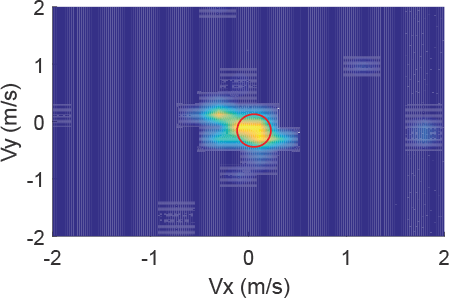
\includegraphics[width=\textwidth]{figures/bvp_stage_1_start}
		\caption{Stage 1: Start}
	\end{subfigure}
	\hfill
	\begin{subfigure}{0.22\textwidth}
		\centering
		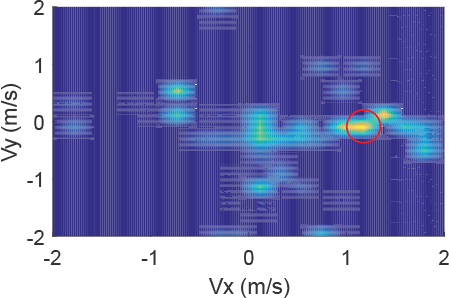
\includegraphics[width=\textwidth]{figures/bvp_stage_2_pushing}
		\caption{Stage 2: Pushing}
	\end{subfigure}
	\hfill
	\begin{subfigure}{0.22\textwidth}
		\centering
		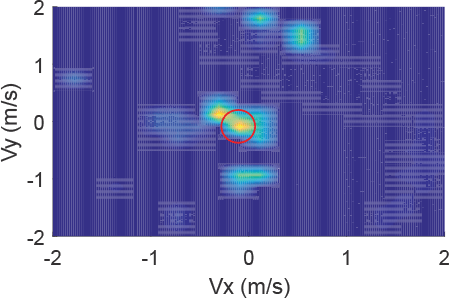
\includegraphics[width=\textwidth]{figures/bvp_stage_3_stop}
		\caption{Stage 3: Stop}
	\end{subfigure}
	\hfill
	\begin{subfigure}{0.22\textwidth}
		\centering
		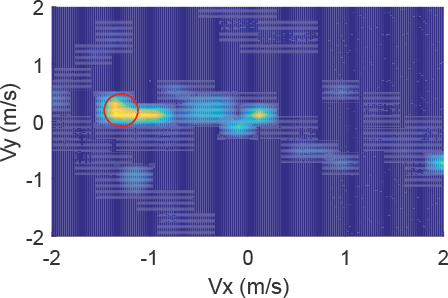
\includegraphics[width=\textwidth]{figures/bvp_stage_4_pulling}
		\caption{Stage 4: Pulling}
	\end{subfigure}
	\caption{A series of slices of a BVP representation of a pushing and pulling gesture, sliced along the time axis. The main velocity component, which represents the movement of the subject's hand, is highlighted with a red circle. This set of images is taken directly from \cite{zheng2019zero}.}
	\label{fig:bvp-example}
\end{figure}

The CSI information, while useful, is also very heavily subjected to various domain factors including, but not limited to, the body composition of the subject, the various objects and their positioning in a room, the direction the subject is facing and the intensity of solar radiation on a given day.
To remedy this, Zheng et al. \cite{zheng2019zero} proposes the use of the Body-coordinate Velocity Profile (BVP), a representation of the CSI which is theoretically independent of domain factors \cite{zheng2019zero}.
A visual representation of BVP can be seen in Figure \ref{fig:bvp-example}.

BVP is derived through a multi-step process where the CSI is first analyzed to capture both the Doppler Frame Shift (DFS) information and to estimate orientation and location of the subject.
The DFS $D$ is then a matrix with dimensions $F \times M$ where $F$ is the number of sampling points in the frequency domain, i.e., the channels, and $M$ the number of transceiver pairs.
The full derivation of DFS from CSI can be seen in Equation 2 of \cite{zheng2019zero}.

The BVP $V$ is derived from the DFS as a discrete $N \times N$ matrix with $N$ being the number of possible values of velocity components decomposed along each axis of the body coordinates.
The authors of \cite{zheng2019zero} use the local body coordinates of the subjects as the origin with the positive x-axis aligning with the orientation of the person.
The full details of the BVP derivation, which are somewhat unnecessary to the understanding of the rest of this thesis, can be found in Section 4 of \cite{zheng2019zero}.

Suffice to say, the BVP representation of a gesture is an $N \times N \times T$ tensor, where $T$ is the time dimension.
This BVP is thus representative of dynamic effects brought by movement of the subject in the DFS representation of the CSI signal and aligned to the orientation and centered on the location of the subject.

\section{Signal-to-Image Transformations}\label{sec:background-signal-to-image}

In this section, we will look into the mathematical formulation of GAFs, MTFs, and RPs.

\subsection{Gramian Angular Fields}

GAFs \cite{wang2015imaging} represents time series in a polar coordinate system and plots the angles in this system.

First, let $X$ be the input signal of length $n$ and $\tilde{X}$ the input rescaled to the interval $[-1, 1]$.

We then represent $\tilde{X}$ in polar coordinates with arguments for the angle $\phi$ and radius $r$ as

\begin{equation}
	\begin{cases}
		\phi = \arccos(\tilde{x}_i), & \tilde{x}_i \in \tilde{X} \\
		r = \frac{t_i}{N}, & t_{i} \in \mathbb{N}
	\end{cases}
\end{equation}
where $t_{i}$ is the timestamp of a given value of $x_i$ and $N$ a constant factor to regularize the span of the polar coordinates.

This is then transformed into the matrix $G$ of size $n \times n$ as

\begin{align}
	G &= \begin{Bmatrix}
		\cos(\phi_1 + \phi_1) & \cdots & \cos(\phi_1 + \phi_n) \\
		\cos(\phi_2 + \phi_1) & \cdots & \cos(\phi_2 + \phi_n) \\
		\vdots                & \ddots & \vdots \\
		\cos(\phi_n + \phi_1) & \cdots & \cos(\phi_n + \phi_n)
	\end{Bmatrix}
	&= \tilde{X}' \cdot \tilde{X} - \sqrt{I - \tilde{X}^2}' \cdot \sqrt{I - \tilde{X}^2}
\end{align}
where $I$ is the unit row vector $[1, 1, \ldots, 1]$.
Defining the inner product $< x,y> = x \cdot y - \sqrt{1 - x^2} \cdot \sqrt{1-y^2}$ results in G being a Gramian matrix with
\begin{equation}
	G = \begin{Bmatrix}
		< \tilde{x}_1, \tilde{x}_1 > & \cdots & < \tilde{x}_1, \tilde{x}_n >\\
		< \tilde{x}_2, \tilde{x}_1 > & \cdots & < \tilde{x}_2, \tilde{x}_n > \\
		\vdots                       & \ddots & \vdots \\
		< \tilde{x}_n \tilde{x}_1 > & \cdots & < \tilde{x}_n, \tilde{x}_n >
	\end{Bmatrix}
\end{equation}

The GAF provides a way to preserve temporal dependencies, with time increasing along the diagonal from the top left to the bottom right.

\subsection{Markov Transition Fields}

MTFs \cite{wang2015imaging} encode the dynamical transition statistics of a time series by representing these transitions as Markov transition probabilities.
Let the input signal $X$ of length $n$ be quantized into $Q$ bins.
Each sample $x_i$ from the input signal is then placed in the corresponding bin $q_j, j \in [1, Q]$.
A matrix $M$ of size $n \times n$ is then constructed where $M_{ij}$ denotes the probability of a transition between bins $q_i \rightarrow q_j$ between two sequential time steps. 
Let the quantile bins that contain the data at timestep $i$ and $j$ be $q_k$ and $q_l$, respectively.
This formally defines $M$ as
\begin{equation}
	M = \begin{Bmatrix}
			w_{kl|x_1 \in q_k, x_1 \in q_l} & \cdots & w_{kl|x_1 \in q_k, x_n \in q_l} \\
			w_{kl|x_2 \in q_k, x_1 \in q_l} & \cdots & w_{kl|x_2 \in q_k, x_n \in q_l} \\
			\vdots                          & \ddots & \vdots                          \\
			w_{kl|x_n \in q_k, x_1 \in q_l} & \cdots & w_{kl|x_n \in q_k, x_n \in q_l}
		\end{Bmatrix}
\end{equation}
$M$ is then an image of size $n \times n$ and can be interpreted as representing the probabilities of any state transitioning into another state over time.

\subsection{Recurrence Plots}

RPs \cite{eckmann1995recurrence} transform the image by representing distances between extracted trajectories in the original time series.
Let the input signal $X$ of length $n$ have extracted trajectories
\begin{equation}
	\vec{x}_i = \left(x_i, x_{i+\tau},\ldots, x_{i+(m-1)\tau}\right), ~ \forall i \ in \{1,\ldots,n-(m-1)\tau\}
\end{equation}
where $m$ is the dimension of the trajectories and $\tau$ is the time delay.
We can then construct the recurrence plot $R$ as the a matrix of size $\left(n - (m-1)\tau\right) \times \left(n - (m-1)\tau\right)$.
Every value in this matrix is defined as the pairwise distance between trajectories, formally
\begin{equation}
	R_{i,j} = \Theta\left(\epsilon - ||\vec{x}_i - \vec{x}_j|| \right),~\forall i,j \in \{1, \ldots, n-(m-1)\tau\}
\end{equation}
where $\epsilon$ is a threshold and $\Theta$ is the Heaviside function
\begin{equation}
	\Theta(x) := \begin{cases}
		1, & x \geq 0\\
		0, & x < 0
	\end{cases}
\end{equation}

This can be interpreted as representing the pairwise distance between trajectories which are above a certain threshold.
